\subsection{Architecture hybride \og orientée états\fg{}}
\label{sec:comm_state}

Dans \cite{Desprat2015a,Desprat2015b}, l'architecture est principalement 
The client-server part is based on a REST (Representa- tional State Transfer) 
architecture [TV10] that benefits from distributed hypermedia systems such as 
our. 


Pros
Easier to maintain
No need to keep a permanent an open connection
Web context: use of HTTP protocol, URI as resource representative, server 
caching


Cons
Bandwidth increasing and latency: client needs to keep locally all the necessary 
data to send the request
  Table 1 resumes the advantages and the drawbacks of a RESTful system. It fits 
  well for web distributed sys- tems even if mobile devices should have limited 
  perfor- mance due to back and forth requests that are energy consuming.
  

nosql database
The rise of the web as a platform encourages the change in data storage for new 
needs like supporting large vol- umes of data (such as 3D data). NoSQL database 
pro- vides dynamic schema and a rich query language API
for data manipulation. Therefore the records can add new information on-the-fly 
facilitating the enrichment of the (3D) objects. In our application the NoSQL 
database is mainly used to maintain persistency of the state of the scenes while a 
user is absent. When the user returns, he/she receives the entire scene 
document. It provides robustness to the system and better experience to the user.

\subsubsection{Spécificité des composants de l'architecture}
Le système présenté repose sur une architecture \acrshort{REST} 
(\acrlong{REST}) concernant les échanges clients-serveur. Cette architecture 
permet de séparer les responsabilités entre le client et le serveur en séparant 
l'\gls{IU} du stockage. \gls{REST} propose une interface uniforme. Cela implique 
que chaque ressource est identifiée et manipulable par des représentation définies 
(modification, suppression). 

Chaque pair correspond a un client (navigateur web) qui contient l'intergiciel 
\gls{P2P} offrant des fonctionnalités limitées, l'interface utilisateur contenant 
l'environnement 3D et un espace de stockage reposant local (IndexedDB).

La persistance long terme est une base de données NoSQL.
NoSQL évite les structures rigides et a tendande à être optimisée pour les grandes 
opérations de lecture. Il est donc possible de stocker des modèles 3D dans une 
base de données, et du à sa flexibilité, aussi tracer d'autres méta données telles 
que les relations entre les différents objets. Dans la base de données, l'accès est 
implicitement supporté de manière distribuée grâce à un langage de requête 
dédiée. La persistence en NoSQL permet d'avoir a un endroit une source de 
données fiable et autoritaire qui permet a un utilisateur de récuperer le bon contenu 
quand il revient sur une scène. La totalité du document contenant la scène est 
envoyé à l'utilisateur lorsqu'il arrive sur une scène.
Le prototype est construit sur l'utilisation de MongoDB.



\subsubsection{Gestion de la session}
Lorsqu'un utilisateur rejoint une session, il suit le déroulement des opérations 
décrit dans la Figure \ref{fig:sequence_state}. 
Dans un premier temps, afin de récupérer les données liées à l'espace de travail, 
le client web de l'utilisateur qui se rend sur une scène récupère 
tous les objets associés à la scène dans la base de données. Les objets de la 
scènes sont renvoyés à l'éditeur pour les afficher. 
Dans un second temps, le système établit les connexions \gls{P2P} entre les 
clients de manière automatique et complète (topologie réseau en maillage 
complet) après avoir récupéré les identifiants des autres utilisateurs auprès du 
serveur de \textit{signaling}. Une fois la connexion établie, chaque collaborateur 
voit son environnement 3D dans l'éditeur mis à jour, indiquant la position du nouvel 
arrivant. Les collaborateurs éditent ensuite la scène 3D qui produit, sur les 
différents objets, des requêtes \gls{CRUD} -- incluant les opérations de translation, 
rotation et homothétie -- destinées au serveur (qui transmet les 
modifications à la base de données) puis aux collaborateurs.
Enfin, dans un dernier temps, lorsque l'utilisateur quitte la scène, il en notifie le 
serveur de \textit{signaling} qui s'occupe d'indiquer aux clients restants, l'abandon 
du client pour qu'ils puissent mettre à jour leur interface en conséquence.

\begin{figure}[ht!]
	\centering
	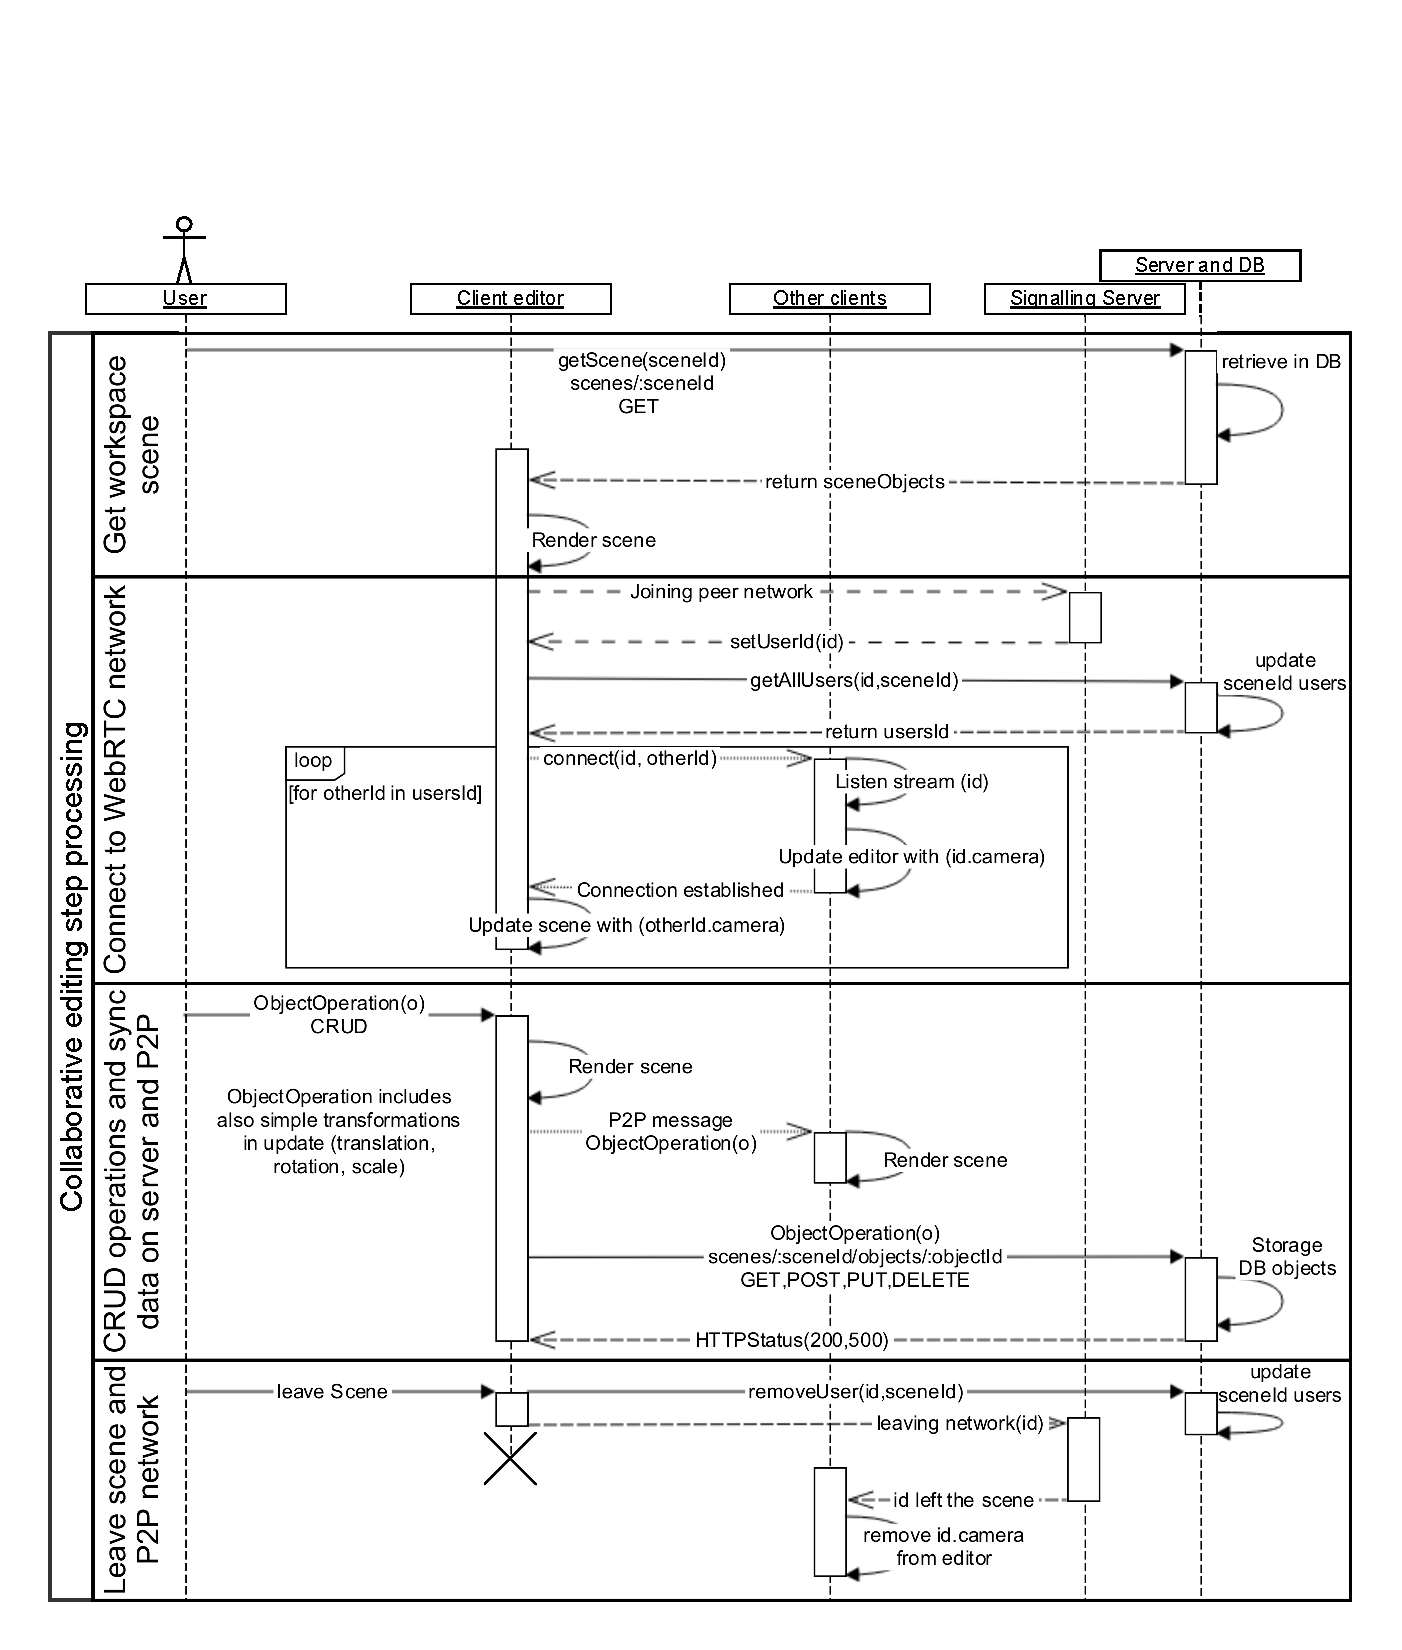
\includegraphics[trim={0 0 0 3cm},clip,width=1\columnwidth]
	{eps/sequence_wscg.eps}
	\caption{Diagramme de séquence de la gestion de la session dans une 
	architecture \og orientée état\fg{}}
	\label{fig:sequence_state}
\end{figure}

%
%We propose to auto connect users on a scene with a We- bRTC connection. As 
%each user send their ID to the database at their arrival, they also retrieve those 
%which where already present on the scene. We are able to cre- ate a full mesh 
%topology network in order to make them communicate the updates.
%
%Even if we have a full mesh topology, the P2P message layer is more similar 
%the 
%star topology. Indeed, the Fig- ure 2 shows the path of a sent message 
%operation 
%on the connection and it is only sent to the one degree neigh- bors of the original 
%broadcaster (the “B” node on the Figure 2).
%
%
%We choose to keep reliable and in order delivery for now. The RTCDataChannel 
%API supports many data types (strings, binary types: Blob, ArrayBuffer. . . ). 
%These types are helpful in a 3D multi user environment to broadcast messages 
%including the objets and their transformations. We tried to limit the amount of 
%data 
%by sending only relevant information but there is actually no particular 
%optimization. The channel can be over- feed when an object is imported then 
%pushed through the network.
%
\subsubsection{Gestion du stockage et structure de données}

Avec une base de données NoSQL utilisant des schémas dynamiques, les 
données sont stockées sous forme de document. Chaque document est 
auto-descriptif et peut contenir des valeurs qui s'imbriquent sous la forme d'une 
structure en arbre hiérarchique. Une collection consiste à grouper des documents, 
équivalent dnas une base de données relationnelle à la notion de table. La base de 
données contient deux types de collections : les scènes et les géométries. Une 
collection de scènes contient des scènes qui sont décrites par leur identifiant et 
les méta-données de l'espace virtuel 3D ainsi que la liste des contributeurs et la 
liste des maillages. Cette liste correspond à une association entre un identifiant de 
maillage, les méta-données de l'objet et l'identifiant d'une géométrie existante. 
Les géométries sont, quant à elles, stockées avec leur identifiant propre et l'objet 
3D complet donné sous le format \gls{JSON}.

Localement, sur chaque client, il existe un stockage relationnel (IndexedDB) pour 
chaque objet 
de la base de donnée récupérée. Cela permet au client de faire des requêtes 
directement dans son espace local si besoin d'ajouter un maillage par exemple. 
C'est également une source pour transférer ses modifications aux autres clients.
Les navigateurs permettent désormais de stocker de quantités de données 
importante localement avec une durée de vie illimitée. 

Les paramètres des opérations fondamentales sur la base de données 
(\gls{CRUD}) sur les collections sont très bien supportés par les requêtes 
\gls{REST}.
\subsubsection{Gestion de la synchronisation et de la cohérence}
L'utilisation d'un algorithme de verrouillage des objets est mises en place pour 
éviter une double sélection et par conséquent les éditions concurrentes. 

Lors de la récupération de la scène, elle est considérée comme cohérente. 
Ensuite, le choix d'avoir des connexions \gls{P2P} ordonnées et fiables ainsi qu'un 
maillage de pair complet, implique que toute donnée envoyée par un pair est 
forcément reçue par les autres. 
\subsubsection{Protocole d'échange}
Les échanges se font à deux niveaux: entre les pairs ainsi qu'entre chaque pair et 
la base de données. Pour le premier niveau, la couche réseau \gls{P2P} est assez 
naïve dans le sens où les connexions sont considérées comme fiables et 
ordonnées, le client n'a alors qu'à publier toutes les modifications qu'il effectue et 
les envoyer à tous les clients (auxquels il est nécessairement connecté).
\subsubsection{Bilan}

La base de données centralisée est beaucoup sollicitée lors des sessions 
collaboratives, ce qui peut mener à une surcharge similaire aux architectures 
uniquement client serveur. 
Chaque pair a une responsabilité importante dans l'envoi de message à tous les 
collaborateurs. La distribution des données devrait être allégée car cette fonction 
de relai peut être lourde pour le fonctionnement du pair. 
La topologie en maillage complet limite le passage à l'échelle car le nombre de 
connexion va croitre de manière exponentielle. 

Les requêtes \gls{CRUD} ne sont pas très expressives concernant le métier. 
Aucune vérification n'est donc effectuée sur la validité des données transmises 
dans cette architecture. De plus, il peut arriver, du fait de latences réseaux que les 
modifications des différents utilisateurs s'entrelacent à l'arrivée et ne rendent pas 
l'intention de l'utilisateur. Cela peut mener à des dé-synchronisations fortes.

L'utilisation d'une solution pessimiste dans un environnement \gls{P2P} peut 
parfois mener à des inter-blocages si un utilisateur quitte la scène sans avoir 
relâché l'objet, c'est à dire, sans en avoir informé la base de données et les autres 
utilisateurs. Même si l'application peut prendre le relais, et permettre la relache du 
verrou au bout d'un certain temps, l'expérience utilisateur peut être dégradée 
pendant cette période.
Le maintient de la cohérence est a peu près garanti dans ce modèle si l'on 
considère un environnement où la fréquence des modifications n'est pas très 
élevée, que tous les clients communique leur horloge local pour établir un 
référentiel de temps concernant les mises à jour. 
%
%Some issues remain in RTCDataChannel API : the com- patibility and 
%interoperability is still not complete be- tween browsers6, some browsers (like 
%Chrome) im- pose a send limit (about 6MB) for the data transmitting through 
%DataConnections and the security of the com- munication is still vulnerable7. 
%The 
%system overview (Figure 4) illustrates the communication architecture topology 
%between the peer clients and server (plus sig- naling).
